
\documentclass[10pt,letterpaper]{article}

\usepackage[letterpaper,margin=0.70in,headheight=22pt,headsep=16pt,footskip=24pt]{geometry}
\usepackage[T1]{fontenc}
\usepackage[utf8]{inputenc}
\usepackage{lmodern}
\usepackage{microtype}
\usepackage{xcolor}
\usepackage{graphicx}
\usepackage{booktabs}
\usepackage{array}
\usepackage{tabularx}
\usepackage{longtable}
\usepackage{amsmath,amssymb}
\usepackage{tikz}
\usetikzlibrary{arrows.meta,positioning,calc,shapes.geometric,decorations.pathreplacing,fit}
\usepackage{enumitem}
\usepackage{fancyhdr}
\usepackage{titlesec}
\usepackage{caption}
\usepackage{listings}
\usepackage{xurl}
\usepackage[hidelinks]{hyperref}
\usepackage{lastpage}
\usepackage{float}
\usepackage{placeins}

% Generated from wvu_beamer_template/styles/beamercolorthemewvu.sty.
% Standalone copy; no Beamer dependency.
\definecolor{wvu-blue}{HTML}{002855}
\definecolor{wvu-gold}{HTML}{EEAA00}
\definecolor{wvu-star-city-blue}{HTML}{9DDAE6}
\definecolor{wvu-safety-blue}{HTML}{0062A3}
\definecolor{wvu-canary}{HTML}{F7DD63}
\definecolor{wvu-sunset}{HTML}{F58672}
\definecolor{wvu-woodburn}{HTML}{8D4638}
\definecolor{wvu-hemlock}{HTML}{6A724F}
\definecolor{wvu-wild-flour}{HTML}{F2E6C2}
\definecolor{wvu-buckskin}{HTML}{B3A169}
\definecolor{wvu-old-gold}{HTML}{7F6310}
\definecolor{wvu-rattler-gray}{HTML}{554741}
\definecolor{wvu-not-quite-white}{HTML}{F7F7F7}
\definecolor{wvu-coopers-gray}{HTML}{BEB7B3}
\definecolor{wvu-seneca-gray}{HTML}{988E8B}
\definecolor{wvu-coal}{HTML}{1C2B39}

\colorlet{PilotProxyRed}{wvu-woodburn}
\colorlet{PilotProxyGray}{wvu-rattler-gray}
\colorlet{PilotProxyBlue}{wvu-blue}
\colorlet{LightGray}{wvu-not-quite-white}
\colorlet{MidGray}{wvu-coopers-gray}
\colorlet{DarkText}{wvu-coal}
\colorlet{GoodGreen}{wvu-hemlock}
\colorlet{WarnGold}{wvu-old-gold}

\renewcommand{\familydefault}{\sfdefault}
\setlength{\parindent}{0pt}
\setlength{\parskip}{5pt}
\renewcommand{\arraystretch}{1.15}
\sloppy
\setlist[itemize]{leftmargin=1.2em,itemsep=2pt,topsep=2pt}
\setlist[enumerate]{leftmargin=1.4em,itemsep=2pt,topsep=2pt}

\titleformat{\section}{\Large\bfseries\color{DarkText}}{}{0pt}{}[\vspace{-3pt}\color{PilotProxyRed}\titlerule]
\titleformat{\subsection}{\large\bfseries\color{DarkText}}{}{0pt}{}
\titleformat{\subsubsection}{\normalsize\bfseries\color{DarkText}}{}{0pt}{}

\newcommand{\code}[1]{\texttt{\detokenize{#1}}}
\newcommand{\apicode}[1]{\texttt{\detokenize{#1}}}
\newcommand{\yes}{\textcolor{GoodGreen}{Yes}}
\newcommand{\no}{\textcolor{PilotProxyGray}{No}}
\newcolumntype{Y}{>{\raggedright\arraybackslash}X}
\newcolumntype{L}[1]{>{\raggedright\arraybackslash}p{#1}}
\newcolumntype{C}[1]{>{\centering\arraybackslash}p{#1}}
\captionsetup{font=small,labelfont=bf}

\lstdefinestyle{shell}{
  basicstyle=\ttfamily\footnotesize,
  breaklines=true,
  columns=fullflexible,
  frame=single,
  rulecolor=\color{MidGray},
  backgroundcolor=\color{LightGray},
  keepspaces=true,
  showstringspaces=false
}
\lstdefinestyle{cstyle}{
  basicstyle=\ttfamily\footnotesize,
  breaklines=true,
  columns=fullflexible,
  frame=single,
  rulecolor=\color{MidGray},
  backgroundcolor=\color{LightGray},
  keepspaces=true,
  showstringspaces=false
}
\lstset{style=shell}

\newcommand{\notebox}[1]{%
  \vspace{4pt}\noindent\fcolorbox{PilotProxyBlue}{LightGray}{%
  \begin{minipage}{0.965\linewidth}%
  \textbf{Note:} #1%
  \end{minipage}}\vspace{4pt}}

\newcommand{\importantbox}[1]{%
  \vspace{4pt}\noindent\fcolorbox{PilotProxyRed}{LightGray}{%
  \begin{minipage}{0.965\linewidth}%
  \textbf{Important:} #1%
  \end{minipage}}\vspace{4pt}}

\newcommand{\field}[1]{\texttt{\detokenize{#1}}}
\newcommand{\dB}{\,\mathrm{dB}}

% Single-sourced numeric specifications (versions, geometry, null_power_ratio range,
% digests). Regenerate with: python tools/generate_doc_specs.py
\input{generated/specs.tex}

\pagestyle{fancy}
\fancyhf{}
\fancyhead[L]{\small PilotProxy-DS001}
\fancyhead[C]{\small CUDA DTV Pilot Detector}
\fancyhead[R]{\small Product Specification}
\fancyfoot[L]{\small PilotProxy-DS001}
\fancyfoot[C]{\small Dylan Gormley}
\fancyfoot[R]{\small Page \thepage\ of \pageref{LastPage}}
\renewcommand{\headrulewidth}{0.8pt}
\renewcommand{\headrule}{\hbox to\headwidth{\color{PilotProxyRed}\leaders\hrule height \headrulewidth\hfill}}
\renewcommand{\footrulewidth}{0.8pt}
\renewcommand{\footrule}{\hbox to\headwidth{\color{PilotProxyRed}\leaders\hrule height \footrulewidth\hfill}}

\title{PilotProxy CUDA DTV Pilot Detector\\Product Specification}
\author{Dylan J. Gormley}
\date{PilotProxy-DS001 \\ October 2026}

\begin{document}
\thispagestyle{fancy}
{\sffamily
\begin{minipage}[t]{0.39\textwidth}
  {\fontsize{24}{26}\selectfont\bfseries\color{PilotProxyRed}PilotProxy}\par
  {\small PilotProxy-DS001, October 2026}
\end{minipage}
\hfill
\begin{minipage}[t]{0.58\textwidth}
  \raggedleft
  {\fontsize{18}{20}\selectfont\bfseries CUDA DTV Pilot Detector}\par
  {\small Product Specification}
\end{minipage}
}

\vspace{0.14in}

\begin{minipage}[t]{0.48\textwidth}
\section*{Introduction}
The purpose of PilotProxy is to measure ATSC 1.0 digital television (DTV) pilot tones with a fixed-point CUDA local-reference power-ratio detector. We use the narrow pilot as a proxy for a DTV data shelf that may lie below the broadband noise floor. The package contains the CUDA kernel, a public C API, Python wrappers, a precomputed ATSC weight bank, and a GNU Radio validation testbench.

The detector core is receiver-independent. The standalone testbench supplies its own reference front end, while the CHIME workflow supplies instrument metadata and packed telescope data through an adapter of its own. This boundary keeps receiver assumptions out of the CUDA kernel. Real-data operation, however, still depends on the instrument.

ATSC A/53 Part 2 specifies that the 8-VSB pilot is approximately 11.3 dB below the average data-signal power \cite{atsc_a53_part2_2011}. We record the positive magnitude of this relationship as \(\mathrm{pilot\_below\_data\_db}=11.3\dB\). Host software uses it to convert one-bin pilot excess to an equivalent DTV data-shelf SNR.

\subsection*{Features}
\begin{itemize}
  \item Fixed-point CUDA detector for ATSC 1.0 pilot excess.
  \item Compile-time 64- or 128-sample detector rows using packed complex
        4+4 bit input, with 128 selected by the shipped CHIME bank.
  \item Three matched-filter terms: target pilot bin, lower reference bin, upper reference bin.
  \item Exact \code{uint64} fine powers per term and fine bin, whose all-bin sums are the target and reference frame powers.
  \item Time-coherent front end: \code{int32} row sums, padded fine
        spectrum, rank-based marker detection.
  \item Synthetic-evaluator detection by an exact integer rational threshold comparison on the host, with no division in that mask path.
  \item Synthetic-evaluator threshold coordinate is DTV shelf SNR in dB.
  \item The corresponding threshold coordinate is a rational power-ratio half-threshold.
  \item GNU Radio ATSC 1.0 waveform generation, audit, AWGN injection, quantization, and SNR evaluation.
  \item Physical-channel helpers and shipped weights for U.S. UHF channels 14-36.
\end{itemize}
\end{minipage}
\hfill
\begin{minipage}[t]{0.48\textwidth}
\section*{PilotProxy Facts Table}
\small
\begin{tabularx}{\linewidth}{|>{\bfseries}L{0.43\linewidth}|Y|}
\hline
\multicolumn{2}{|c|}{\bfseries Core Specifics}\\ \hline
Package version & \ppPackageVersion \\ \hline
Kernel core version & \ppKernelCoreVersion \\ \hline
Primary function & Measure ATSC 1.0 pilot excess and estimate the corresponding data-shelf SNR \\ \hline
Input data & Packed complex int4, one complex sample per \code{int8_t} \\ \hline
Detector window & 64 or 128 packed complex samples; shipped CHIME bank: \ppDetectorWindowSamples \\ \hline
Weight terms & 3: target, lower reference, upper reference \\ \hline
Reference bins & Two total reference bins \\ \hline
Raw statistic & \(F=2P_t/(P_{r1}+P_{r2})\) \\ \hline
Raw/basic pilot excess & \(\rho=F-1\); positive raw excess begins at \(F>1\) \\ \hline
Kernel outputs & \code{mask} (deployment; 1 = reject), \code{uint64} fine powers and frame powers, \code{int32} row sums \\ \hline
Power accumulation & \code{uint64} \\ \hline
\multicolumn{2}{|c|}{\bfseries User-Facing Controls}\\ \hline
Target selection & \code{physical_channel} or \code{dtv_pilot_mhz} selects precomputed weights \\ \hline
Frame size & Matched to the correlator frame; CHIME F-engine target $2^{14}$ \\ \hline
Synthetic threshold & Shelf SNR in dB; converted by evaluator host software \\ \hline
\multicolumn{2}{|c|}{\bfseries Reference Testbench}\\ \hline
Reference ADC rate & 800 MS/s real input \\ \hline
Reference band & 400-800 MHz \\ \hline
PFB & 4-tap, 2048-point real-input PFB \\ \hline
Usable coarse channels & 1024 positive-frequency channels \\ \hline
Coarse-channel spacing & 390.625 kHz \\ \hline
Detector-bin width & \ppDetectorBinHz\ Hz \\ \hline
Default physical channel & 14; 470--476 MHz band, pilot at 470.309441 MHz \\ \hline
Shipped weight range & Physical channels 14-36 \\ \hline
\multicolumn{2}{|c|}{\bfseries Implementation}\\ \hline
CUDA dot-product path & DP4A production path; scalar integer validation path \\ \hline
Default block threads & 64 \\ \hline
Default grid cap & 4096 blocks \\ \hline
Default weight placement & Shared-memory preload enabled \\ \hline
Execution policy & Device-affine, default stream \\ \hline
\end{tabularx}
\end{minipage}

\vfill
{\small\color{PilotProxyGray}The runtime decision uses the rank-based fine score. The archive $F>\mu_0$ flag and the synthetic thresholds are diagnostics. Measure performance on the target system.}

\newpage
\tableofcontents
\newpage

\section{General Description}

The DTV data shelf occupies most of a nominal 6 MHz channel, but the ATSC pilot is narrow. Therefore, we measure the pilot against two nearby reference bins and use that excess to estimate the equivalent data-shelf SNR. This estimate is conditional on the stated bandwidth, pilot-to-data relationship, and pilot-capture efficiency.

The CUDA kernel implements only the fixed-point measurement. It receives a row-major detector matrix and three packed weight vectors. It returns the exact \code{uint64} fine powers of the three terms and the frame powers, their all-bin sums. The fused mask entries also return the per-frame mask bit of the fine decision. Host software applies the coarse threshold comparison in exact integer arithmetic and supplies the ATSC frequencies, dB conversions, receiver geometry, and physical-channel interpretation.


\begin{figure}[H]
\centering
% Standalone validation flow.
% This file is the one source of the diagram. It is \input by PilotProxy_DS001
% (Data Sheet) and PilotProxy_UG001 (User Guide) and rendered to
% validation_flow.svg for docs/USAGE.md. It needs the tikz libraries
% arrows.meta and positioning, and the colors PilotProxyBlue (WVU blue) and
% LightGray (WVU not-quite-white) defined by the host document, or by
% validation_flow_standalone.tex when the svg is rendered. The svg must be
% rendered again after each edit:
%   cd docs/figures && pdflatex validation_flow_standalone.tex \
%     && pdftocairo -svg validation_flow_standalone.pdf validation_flow.svg
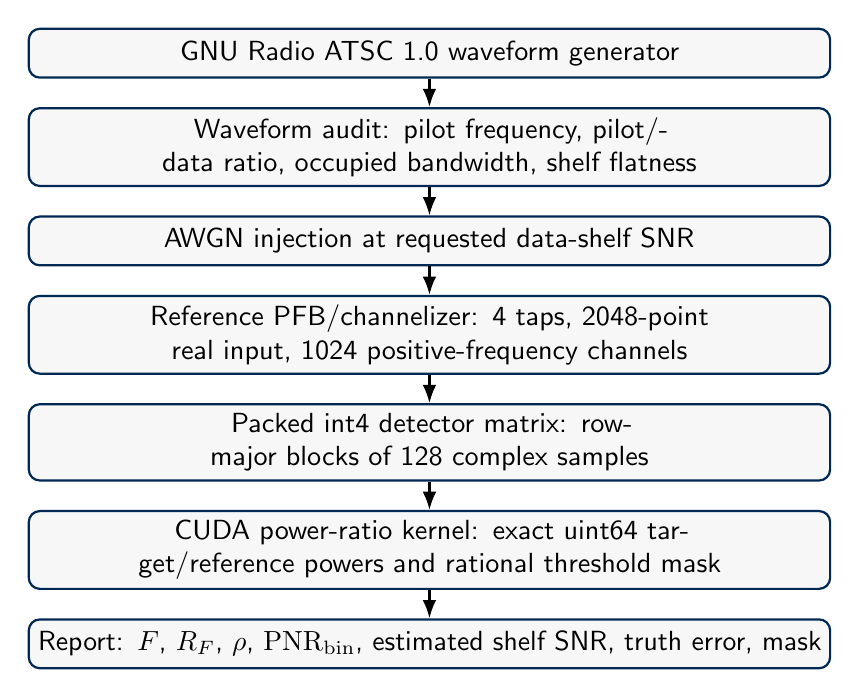
\begin{tikzpicture}[node distance=0.36cm,>=Latex]
\tikzstyle{block}=[rectangle,rounded corners,draw=PilotProxyBlue,thick,fill=LightGray,minimum height=0.62cm,text width=0.82\linewidth,align=center]
\node[block] (a) {GNU Radio ATSC 1.0 waveform generator};
\node[block,below=of a] (b) {Waveform audit: pilot frequency, pilot/data ratio, occupied bandwidth, shelf flatness};
\node[block,below=of b] (c) {AWGN injection at requested data-shelf SNR};
\node[block,below=of c] (d) {Reference PFB/channelizer: 4 taps, 2048-point real input, 1024 positive-frequency channels};
\node[block,below=of d] (e) {Packed int4 detector matrix: row-major blocks of 128 complex samples};
\node[block,below=of e] (f) {CUDA power-ratio kernel: exact uint64 target/reference powers and rational threshold mask};
\node[block,below=of f] (g) {Report: $F$, $R_F$, $\rho$, $\mathrm{PNR}_{\mathrm{bin}}$, estimated shelf SNR, truth error, mask};
\draw[->,thick] (a) -- (b);
\draw[->,thick] (b) -- (c);
\draw[->,thick] (c) -- (d);
\draw[->,thick] (d) -- (e);
\draw[->,thick] (e) -- (f);
\draw[->,thick] (f) -- (g);
\end{tikzpicture}

\caption{Standalone validation flow. Here, the reference front end of the package connects a generated ATSC waveform to the same packed-input detector contract used by the CUDA kernel.}
\label{fig:validation_flow}
\end{figure}

\begin{figure}[H]
\centering
% Shared diagram of the implemented Kotekan mask path. Requires arrows.meta,
% positioning, calc and the PilotProxy color names from the host document.
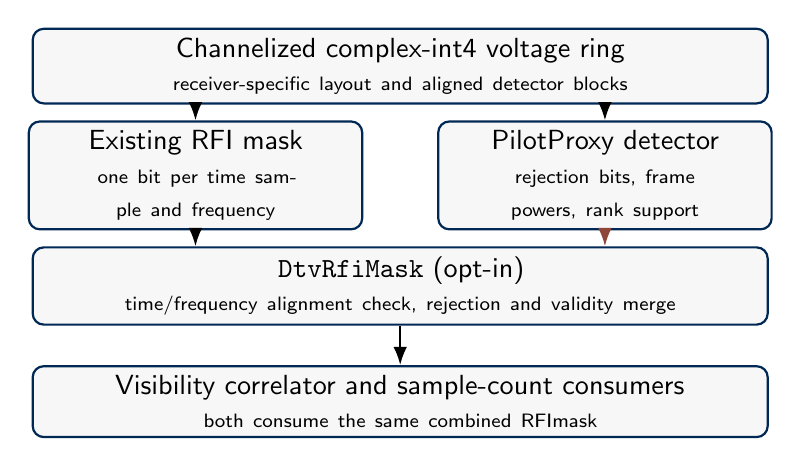
\begin{tikzpicture}[node distance=0.5cm,>=Latex,
  blk/.style={rectangle,rounded corners,draw=PilotProxyBlue,thick,fill=LightGray,
              minimum height=0.75cm,align=center,text width=4.0cm},
  wide/.style={blk,text width=9.1cm}]

\node[wide] (voltage) {Channelized complex-int4 voltage ring\\
  \scriptsize receiver-specific layout and aligned detector blocks};
\node[blk] (rfi) at ($(voltage.south)+(-2.6,-0.9)$)
  {Existing RFI mask\\ \scriptsize one bit per time sample and frequency};
\node[blk] (detector) at ($(voltage.south)+(2.6,-0.9)$)
  {PilotProxy detector\\ \scriptsize rejection bits, frame powers, rank support};
\node[wide,below=1.8cm of voltage] (combine)
  {\texttt{DtvRfiMask} (opt-in)\\
   \scriptsize time/frequency alignment check, rejection and validity merge};
\node[wide,below=of combine] (consumers)
  {Visibility correlator and sample-count consumers\\
   \scriptsize both consume the same combined RFImask};

\draw[->,thick] (voltage.south -| rfi.north) -- (rfi.north);
\draw[->,thick] (voltage.south -| detector.north) -- (detector.north);
\draw[->,thick] (rfi.south) -- (combine.north -| rfi.south);
\draw[->,thick,PilotProxyRed] (detector.south) -- (combine.north -| detector.south);
\draw[->,thick] (combine) -- (consumers);
\end{tikzpicture}

\caption{Mask path implemented in Kotekan. Here, the detector reads the
voltage ring and writes a rejection bit, frame powers, and optional rank
support for each aligned block. The opt-in \code{DtvRfiMask} stage intersects
those decisions with the existing RFImask, and both the visibility and
sample-count consumers use the resulting mask. The diagnostic include for
CHIME is detect-only. Receiver qualification is described in
\code{docs/OPERATOR_HANDOFF.md}.}
\label{fig:system_context}
\end{figure}


\section{Signal Definitions}

\subsection{Raw Local-Reference Power Ratio}

For one evaluated frame, the kernel produces three frame powers:
\begin{equation}
  P_t,\qquad P_{r1},\qquad P_{r2},\qquad
  P_n=\sum_{f}S[n,f],
\end{equation}
each the exact \code{uint64} all-bin sum of that term's fine power spectrum
\(S[n,f]\) (Section~\ref{ssec:fine}). The target term \(P_t\) is centered on the ATSC pilot. The lower and upper reference terms, \(P_{r1}\) and \(P_{r2}\), sample the nearby non-pilot floor. We form the raw power ratio as
\begin{equation}
  \boxed{F=\frac{2P_t}{P_{r1}+P_{r2}}.}
\end{equation}
The fine-transform length cancels in this ratio. The library forms no ratio,
so host code receives the three exact powers and must use
\(F=2P_t/(P_{r1}+P_{r2})\). Using \(P_t/(P_{r1}+P_{r2})\) would omit the factor of two in the detector definition.

\subsection{Pilot Excess and PNR}

The raw power ratio level is:
\begin{equation}
  R_F=10\log_{10}F.
\end{equation}
This level is not the physical pilot-to-noise ratio because \(F=1\) is the uncorrected no-excess point. We define the corresponding raw pilot excess as
\begin{equation}
  \boxed{\rho=F-1.}
\end{equation}
Physical pilot excess uses the exact packed-weight normalization,
\(\mu_0=2\lVert w_t\rVert^2/(\lVert w_{r1}\rVert^2+\lVert w_{r2}\rVert^2)\):
\begin{equation}
  e=F/\mu_0-1,\qquad
  \boxed{\mathrm{PNR}_{\mathrm{bin},dB}=10\log_{10}e.}
\end{equation}
The raw excess \(\rho\) is diagnostic only. For \(e\leq0\), the logarithm is
undefined, and JSON reports encode it as \code{null}, while the signed linear
excess remains available. Here, \(\mu_0\) is a ratio of expected powers under
flat noise, which differs from the finite-sample expectation of the random
ratio \(F\).

\subsection{DTV Shelf SNR}

We define the DTV data-shelf SNR as the ATSC data-and-sync shelf power spectral density relative to the non-DTV noise floor. The pilot is not part of the shelf numerator. For the standard conversion, we compute
\begin{equation}
  \boxed{\mathrm{SNR}_{\mathrm{shelf},dB}=
  \mathrm{PNR}_{\mathrm{bin},dB}
  -10\log_{10}\left(\frac{B_{\mathrm{DTV}}}{B_{\mathrm{bin}}}\right)
  +\mathrm{pilot\_below\_data\_db}
  -10\log_{10}(\eta_p).}
\end{equation}
The default constants are:
\begin{equation}
 B_{\mathrm{DTV}}=6\,\mathrm{MHz},\quad
 B_{\mathrm{bin}}=3051.7578125\,\mathrm{Hz},\quad
 \mathrm{pilot\_below\_data\_db}=11.3\dB,
 \quad \eta_p=1.0.
\end{equation}
For these constants, the bandwidth spreading term is
\begin{equation}
  10\log_{10}\left(\frac{6\times 10^6}{\ppDetectorBinHz}\right)=\ppBandwidthSpreadDb\dB.
\end{equation}

\subsection{Time-Coherent Fine Statistic}
\label{ssec:fine}

The time-coherent front end replaces the reduction after the dot product.
Instead of squaring the dot product of each window and summing incoherently
over all rows, the windows are integrated coherently, and only the feed sum
remains incoherent. For \(W=128\) windows, this recovers up to
\ppCoherentGainDb~dB of deflection sensitivity (\(10\log_{10}\sqrt{W}\), less
scalloping). For each weight term \(n\in\{t,r1,r2\}\) and detector row \(m\),
the front end returns the complex dot product
\begin{equation}
  z[n,m]=\sum_{k=0}^{K-1} w_n[k]\,x_m[k]
  \qquad(\text{exact \code{int32} components}).
\end{equation}
In the fine stage, the rows of each term are reshaped to
\([N_{\mathrm{streams}},\,W]\) with \(W=\mathrm{frame\_size\_samples}/K\)
windows per stream, the frozen fixed-point FFT (\code{fxfft256_v1}) is applied
along the window axis with \(\times\ppFinePadFactor\) zero padding, and the
result is summed incoherently over streams:
\begin{equation}
  S[n,b]=\sum_{\mathrm{streams}}\bigl|\mathrm{FFT}_{\mathrm{pad}}(z[n,\cdot])[b]\bigr|^2,
  \qquad
  \boxed{F_2[b]=\frac{2\,S[t,b]}{S[r1,b]+S[r2,b]},}
\end{equation}
for \(b=0,\ldots,\ppFineNumBins-1\) fine bins of width \ppFineBinHz\ Hz
(the detector-bin width divided by \ppFineNumBins). The reduction is
coherent in time over one frame and incoherent over streams and frames.

No inter-window phase corrector is required. The steering frequency of each
term is an integer bin of the \(K\)-sample window, so the window-to-window
phase of an offset tone passes through stage 1 exactly
(\(e^{2\pi i c_n j}=1\) for integer bin \(c_n\)). The omitted intra-window fine
rotation \(e^{-2\pi i kb/(\mathrm{pad}\cdot WK)}\) is the window capture factor
documented in \code{docs/METHOD_SPEC.md} (\(\mathrm{sinc}^2\) scalloping:
\ppCaptureLossThreeHundredDb~dB at 300\,Hz, at most \ppCaptureLossEdgeDb~dB at
the fine-span edge).

The frame powers of the coarse statistic are defined as the all-bin sums of
this spectrum, \(P_n=\sum_b S[n,b]\). Thus, \(F\) is exactly the all-bin
marginal of the fine spectrum, with no second power path. Each product stores
both, and the readers check \(P_n=\sum_b S[n,b]\) exactly. Since the rounded
fixed-point transform does not conserve energy exactly, \(P_n\) differs
from \(\mathrm{pad}\cdot W\sum_m|z[n,m]|^2\). The two agree to a
median relative \(3\times10^{-6}\) on archive frames and depart by up to about
2 percent on near-empty frames. The runtime fine decision compares the largest
marker-bin ratio with a calibrated multiple of a bulk order statistic. Any-bin
diagnostic tests are recomputed in post-processing from the stored fine
powers. The stored fields are specified in \code{docs/PRODUCT_SCHEMA.md}.

\subsection{Distributional Statement (Null Hypothesis)}
\label{ssec:dist}

We assume, under the null hypothesis, that there is no pilot, that the
spectrum is locally flat over the three terms, and that the channelized noise
is circular complex Gaussian. With these assumptions, the dot product \(z_n\)
of each term is complex Gaussian, so each per-row power \(|z_n|^2\) is a
scaled \(\chi^2_2\) variable, and the three terms are independent because they
sample disjoint detector bins. For one detector row with equal term norms,
write \(|z_t|^2 = \tfrac{s}{2}U\) and
\(|z_{r1}|^2+|z_{r2}|^2 = \tfrac{s}{2}V\) with \(U\sim\chi^2_2\),
\(V\sim\chi^2_4\), and a common scale \(s\). Then
\begin{equation}
F_{\mathrm{row}}
= \frac{2\,|z_t|^2}{|z_{r1}|^2+|z_{r2}|^2}
= \frac{2U}{V}
= \frac{U/2}{V/4}
\;\sim\; F(2,4),
\end{equation}
which is the F distribution with \((2,4)\) degrees of freedom, a 2-dof power
over the mean of two independent 2-dof powers. This F law is an idealized
reference only, and it is not claimed for the production detector or for its
rank-normalized fine score.

The ideal frame statistic sums powers over \(M\) rows before the ratio
(\code{all_rows_summed_before_ratio}), which replaces \((2,4)\) by
\((2M,\,4M)\). That is, under the same assumptions, \(F \sim F(2M, 4M)\). The
frame powers are the all-bin sums of the fine spectrum, and an exact transform
would make them \(\mathrm{pad}\cdot W\) times the row sums in every term, so
the same distribution holds up to the fixed-point rounding of the transform.
The per-row \(F(2,4)\) has mean \(4/(4-2)=2\) and a heavy right tail, while
the frame statistic with \(M=\ppChimeRowsPerFrame\) rows is tightly
concentrated, with \(\mathrm{E}[F(2M,4M)] = 4M/(4M-2) \to 1\). The zero point
\(\mu_0\) of the mask is the ratio of expectations \(2 n_t/(n_{r1}+n_{r2})\),
evaluated with the exact quantized norms, and it is the value approached by
the concentrated frame statistic. The mask itself relies on no distributional
form, since it is an exact integer comparison against \(\mu_0\).

With unequal reference norms, the denominator is a weighted sum of two
\(\chi^2_2\) terms, and the \(4M\)-dof form is a Satterthwaite-style
approximation. Correlated or non-Gaussian interference violates the
assumption of row independence. Each fine bin repeats the construction over
\(N_{\mathrm{s}}\) streams, so that
\(F_2[b] \sim F(2N_{\mathrm{s}},\,4N_{\mathrm{s}})\) on independent bins under
\(H_0\). The fine score, however, normalizes marker ratios by a bulk order
statistic. This normalization does not by itself set a false-alarm rate, and
its calibration requires an appropriate independent noise population.

\begin{figure}[H]
\centering
% Shared architecture diagram: detector datapath in the two-stage
% channelizer (filterbank) view.
% Single source of truth -- \input by PilotProxy_DS001 (Data Sheet) and
% PilotProxy_UG001 (User Guide); render detector_datapath.svg for markdown
% use with detector_datapath_standalone.tex. Requires tikz libraries
% arrows.meta + positioning + calc + decorations.pathreplacing, and the
% colors PilotProxyBlue, PilotProxyRed, PilotProxyGray, LightGray from the host document
% (or the standalone wrapper).
% Re-render the svg after editing:
%   cd docs/figures && pdflatex detector_datapath_standalone.tex \
%     && pdftocairo -svg detector_datapath_standalone.pdf detector_datapath.svg
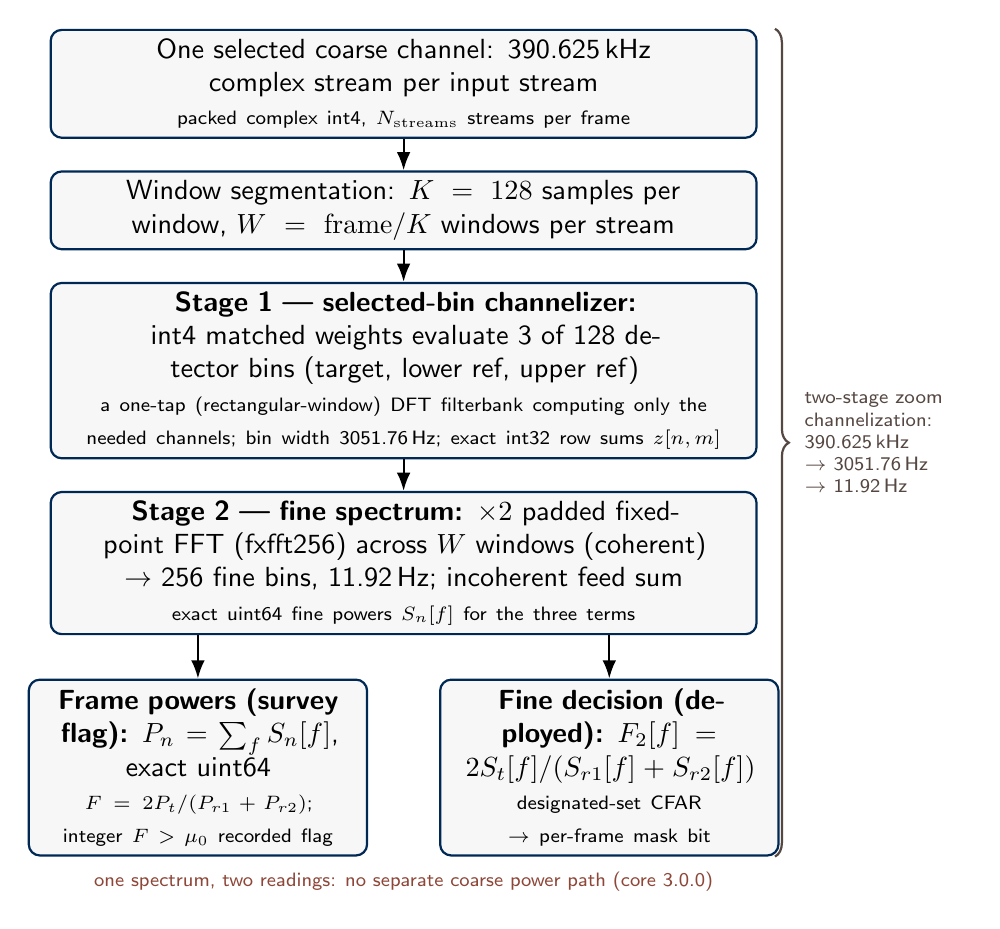
\begin{tikzpicture}[node distance=0.40cm,>=Latex,
  blk/.style={rectangle,rounded corners,draw=PilotProxyBlue,thick,fill=LightGray,
              minimum height=0.62cm,align=center,text width=0.72\linewidth},
  half/.style={rectangle,rounded corners,draw=PilotProxyBlue,thick,fill=LightGray,
               minimum height=0.62cm,align=center,text width=0.335\linewidth}]

\node[blk] (in) {One selected coarse channel: 390.625\,kHz complex stream
  per input stream\\ \scriptsize packed complex int4,
  $N_{\mathrm{streams}}$ streams per frame};
\node[blk,below=of in] (seg) {Window segmentation: $K=128$ samples per
  window, $W=\mathrm{frame}/K$ windows per stream};
\node[blk,below=of seg] (s1) {\textbf{Stage 1 --- selected-bin
  channelizer:} int4 matched weights evaluate 3 of 128 detector bins
  (target, lower ref, upper ref)\\ \scriptsize a one-tap
  (rectangular-window) DFT filterbank computing only the needed channels;
  bin width 3051.76\,Hz; exact int32 row sums $z[n,m]$};
\node[blk,below=of s1] (s2) {\textbf{Stage 2 --- fine spectrum:}
  $\times 2$ padded fixed-point FFT (fxfft256) across $W$ windows
  (coherent) $\to$ 256 fine bins, 11.92\,Hz; incoherent feed sum\\
  \scriptsize exact uint64 fine powers $S_n[f]$ for the three terms};
\node[half,anchor=north east] (v1) at ($(s2.south)+(-0.45,-0.55)$)
  {\textbf{Frame powers (survey flag):} $P_n=\sum_f S_n[f]$, exact
  uint64\\ \scriptsize $F = 2P_t/(P_{r1}+P_{r2})$; integer $F>\mu_0$
  recorded flag};
\node[half,anchor=north west] (v2) at ($(s2.south)+(0.45,-0.55)$)
  {\textbf{Fine decision (deployed):}
  $F_2[f]=2S_t[f]/(S_{r1}[f]+S_{r2}[f])$\\
  \scriptsize designated-set CFAR $\to$ per-frame mask bit};

\draw[->,thick] (in) -- (seg);
\draw[->,thick] (seg) -- (s1);
\draw[->,thick] (s1) -- (s2);
\draw[->,thick] (s2.south -| v1.north) -- (v1.north);
\draw[->,thick] (s2.south -| v2.north) -- (v2.north);
\node[font=\scriptsize\color{PilotProxyRed},align=center]
  at ($(s2.south |- v2.south)+(0,-0.32)$)
  {one spectrum, two readings: no separate coarse power path (core 3.0.0)};

\coordinate (brx) at ([xshift=0.22cm]s1.east);
\draw[decorate,decoration={brace,amplitude=5pt},thick,PilotProxyGray]
  (brx |- in.north) -- (brx |- v2.south)
  node[midway,right=7pt,font=\scriptsize\color{PilotProxyGray},align=left,
       text width=2.0cm]
  {two-stage zoom channelization:\\ 390.625\,kHz\\ $\to$ 3051.76\,Hz\\
   $\to$ 11.92\,Hz};
\end{tikzpicture}

\caption{Detector datapath in the filterbank view. Here, stage 1 is a
critically sampled DFT filterbank with a rectangular (one-tap) prototype,
evaluated only at the three needed channels through the int4 matched weights.
The window-axis FFT is the second stage of a standard two-stage zoom
channelization and refines the selected detector bin from \ppDetectorBinHz\ Hz
to \ppFineBinHz\ Hz. The fine path is an implemented, inactive decision
candidate. Coherent window integration recovers up to \ppCoherentGainDb~dB of
deflection sensitivity over the all-incoherent reduction, and the
designated-set CFAR can form a per-frame candidate mask bit with a
deterministic FFT that is bit-exact between host and device. The frame powers
are the all-bin sums of the same fine powers and supply the archive
$F>\mu_0$ rejection flag, and the coarse statistic has no second power path
(\code{docs/DESIGN_DECISIONS.md}).}
\label{fig:detector_datapath}
\end{figure}


\begin{figure}[H]
\centering
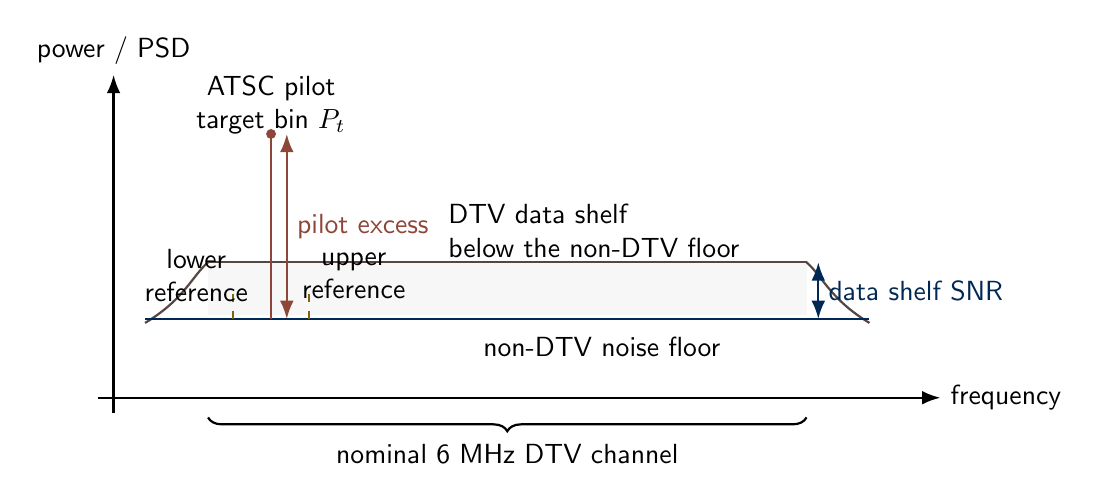
\begin{tikzpicture}[x=1.0cm,y=1.0cm,>=Latex]
  \draw[->,thick] (-0.2,0) -- (10.5,0) node[right]{frequency};
  \draw[->,thick] (0,-0.2) -- (0,4.1) node[above]{power / PSD};
  \draw[fill=LightGray,draw=none] (1.2,1.05) rectangle (8.8,1.72);
  \draw[thick,PilotProxyGray] (1.2,1.72) -- (8.8,1.72);
  \draw[thick,PilotProxyGray] (0.4,0.95) .. controls (0.9,1.25) and (1.0,1.55) .. (1.2,1.72);
  \draw[thick,PilotProxyGray] (8.8,1.72) .. controls (9.0,1.55) and (9.1,1.25) .. (9.6,0.95);
  \draw[thick,PilotProxyBlue] (0.4,1.0) -- (9.6,1.0);
  \draw[thick,PilotProxyRed] (2.0,1.0) -- (2.0,3.35);
  \draw[fill=PilotProxyRed,draw=PilotProxyRed] (2.0,3.35) circle (0.055);
  \draw[dashed,thick,WarnGold] (1.52,1.0) -- (1.52,1.35);
  \draw[dashed,thick,WarnGold] (2.48,1.0) -- (2.48,1.35);
  \draw[<->,thick,PilotProxyRed] (2.20,1.0) -- (2.20,3.35) node[midway,right]{pilot excess};
  \draw[<->,thick,PilotProxyBlue] (8.95,1.0) -- (8.95,1.72) node[midway,right]{data shelf SNR};
  \draw[decorate,decoration={brace,mirror,amplitude=5pt},thick] (1.2,-0.25) -- (8.8,-0.25)
    node[midway,below=6pt]{nominal 6 MHz DTV channel};
  \node[align=center] at (2.0,3.72) {ATSC pilot\\target bin $P_t$};
  \node[align=center] at (1.05,1.55) {lower\\reference};
  \node[align=center] at (3.05,1.55) {upper\\reference};
  \node[align=left] at (6.1,2.12) {DTV data shelf\\below the non-DTV floor};
  \node[align=left] at (6.2,0.65) {non-DTV noise floor};
\end{tikzpicture}
\caption{Signal definitions used by the detector. The kernel compares the target pilot bin with two local reference bins. Host software then converts the measured one-bin excess to an equivalent 6 MHz data-shelf SNR under the stated calibration constants.}
\label{fig:spectrum_definitions}
\end{figure}


\section{Threshold Interpretation}

For synthetic threshold tests, the user supplies \code{threshold_data_shelf_snr_db}. Host software converts this shelf-SNR threshold to the raw power ratio coordinate and then to a rational half-threshold, which it applies to the integer frame powers:

\begin{align}
\mathrm{PNR}_{\mathrm{bin,thr},dB} &= S_{\mathrm{shelf,thr},dB} - \mathrm{pilot\_below\_data\_db} + 10\log_{10}(B_{\mathrm{DTV}}/B_{\mathrm{bin}})+10\log_{10}(\eta_p),\\
\rho_{\mathrm{thr}} &= 10^{\mathrm{PNR}_{\mathrm{bin,thr},dB}/10},\\
F_{\mathrm{thr}} &= 1+\rho_{\mathrm{thr}},\\
T_{\mathrm{half}} &= \frac{F_{\mathrm{thr}}}{2}=\frac{N_{\mathrm{half}}}{D_{\mathrm{half}}}.
\end{align}
The host evaluates, in exact integer arithmetic:
\begin{equation}
  P_t D_{\mathrm{half}} > N_{\mathrm{half}}(P_{r1}+P_{r2}).
\end{equation}
Exact equality is not counted as a detection, since the synthetic threshold path and the CHIME positive-excess path both use a strict greater-than comparison.


\notebox{We independently recomputed the following example from the checked-in conversion code. For a \(-26\dB\) shelf-SNR threshold and the shipped reference geometry, \(\mathrm{PNR}_{\mathrm{bin}}=-4.363988\dB\), \(F_{\mathrm{thr}}=1.36610123\), and \(T_{\mathrm{half}}\approx0.68305\).}

\section{Channel and Frequency Support}

The shipped weight bank covers U.S. physical channels 14 through 36. The eCFR assigns channel 14 to 470--476 MHz and channel 36 to 602--608 MHz \cite{ecfr_73603}. Following the ATSC pilot offset, the default channel-14 target is 470.309441 MHz.

\begin{longtable}{|C{0.13\linewidth}|C{0.18\linewidth}|C{0.20\linewidth}|C{0.33\linewidth}|}
\hline
\textbf{Physical channel} & \textbf{Lower edge} & \textbf{Pilot} & \textbf{Coarse index: ascending reference / shipped CHIME}\\ \hline
14 & 470.000 MHz & 470.309441 MHz & 179 / 843, lower reference edge wrapped\\ \hline
21 & 512.000 MHz & 512.309441 MHz & 287 / 735\\ \hline
36 & 602.000 MHz & 602.309441 MHz & 517 / 505\\ \hline
\end{longtable}

The first index is the standalone ascending-frequency reference coordinate. The second is the post-Nyquist-zone-normalization coordinate stored in the shipped CHIME manifest and printed by \code{pilot-proxy list-channels}. The nominal references are two detector bins below and above the target. In the shipped DC-centered bank, physical channel 14 is the only adaptive case. Its target lies near a coarse-channel boundary, so the generated layout wraps the lower reference across the circular coarse-channel spectrum while preserving the two-bin offset, and \code{list-channels} prints the matching placement \code{NOTE}. No shipped channel collides with, or shifts around, the forbidden coarse-channel DC tone. Detection and validation reports copy the selected manifest row into \field{selected_weight_layout}, so this placement remains visible in each result.

\section{Receiver Integration Contract}

The CUDA detector core does not interpret receiver metadata. A receiver adapter must supply the following metadata and arrays above the kernel boundary:
\begin{itemize}
  \item \code{DetectorCoreProfile}: locked kernel contract, which covers the
        selected \(K\in\{64,128\}\), \(N=3\), int4 packed input, uint64
        fine and frame powers, and no threshold input.
  \item \code{ReceiverProfile}: RF band, channelizer geometry, Nyquist zone, baseband frame convention (\field{baseband_frame.channel_center_normalized}), frame size, input-stream count, quantization defaults, detector-bin ENBW, and pilot-capture efficiency.
  \item \code{stream_map}: stream-index metadata for feed, polarization, beam, or other receiver paths.
  \item \code{check-profile}, \code{check-layout}, \code{make-weights}, and \code{chime-run} consume the applicable profile or stream-map records. The standalone \code{detect} command selects shipped weights from its sidecar or channel flag, while \code{evaluate-snr} uses the fixed testbench geometry.
\end{itemize}

After this adaptation, the kernel receives only packed rows and packed weights, and it writes uint64 powers and a mask. For one selected DTV channel, the adapter constructs
\begin{equation}
N_{\mathrm{rows}} = N_{\mathrm{input\ streams}}\,
\frac{\mathrm{frame\_size\_samples}}{K}.
\end{equation}
The default combine mode is an incoherent power sum over streams. We sum the powers before forming the statistic:
\begin{equation}
F = \frac{2\sum_r P_{t,r}}{\sum_r P_{r1,r}+\sum_r P_{r2,r}},
\end{equation}
where \(r\) indexes detector rows. The result schema names this rule \code{all_rows_summed_before_ratio}. Per-stream packing remains available for integration diagnostics, but the combined detection path forms one \(F\) only after summing all selected rows.

The frame size is set by the correlator. The adapter matches the frame of the correlator, and the kernel requires that value to be a positive multiple of the profile-selected \(K\). The checked-in \code{chime_dtv_fengine} receiver profile selects \(K=\ppDetectorWindowSamples\) and uses \(2^{14}=16384\) channelized samples per input stream, the frame of the CHIME F-engine upgrade that this integration is designed for. It also declares the frame-verified DC-centered baseband convention (\field{baseband_frame.channel_center_normalized}=0.0), validated against archived CHIME baseband. For this profile and one selected coarse channel, \(\ppChimeStreams\times\ppWindowsPerStream=\ppChimeRowsPerFrame\) detector rows form one frame. The CHORD profiles select \(K=64\) with an 8192-sample frame, and both profile families keep 128 windows per stream for the frozen fine transform. These frame sizes are integration contracts and make no claim about a correlator frame deployed everywhere. The software does not infer one universal value from HDF5 metadata. \code{chime-run} accepts an explicit per-run frame-size override, while \code{chime-scan} takes \code{nfft} from the PilotProxy CHIME instrument configuration. Operators must verify and record the resolved value for each real-data product.

\section{Result Schema and Mask Convention}

Detector and synthetic SNR-evaluator JSON outputs carry a versioned \field{result_schema} object with \code{schema_version=pilotproxy_result_schema_v2}. This object records the statistic definitions, layout metadata, calibration constants, threshold fields, fixed-point contract, and mask convention needed to interpret those results. Audit, quantization, summary, injection, and CHIME products use their own documented top-level schemas instead of this object.

The fixed-point contract records:
\begin{itemize}
  \item \field{detector_window_samples} equal to the profile-selected 64 or
        128 (128 for the shipped CHIME bank);
  \item \field{reference_offset_bins=2} as the nominal value, with \field{skipped_guard_bins=1} and adaptive placement metadata copied from the weight manifest;
  \item \field{packed_complex_bits=8};
  \item \field{sample_bits_per_component=4};
  \item \field{power_accumulator=uint64}.
\end{itemize}

For products that average masked data, we use exclusion masking:
\begin{equation}
\bar{P}_{\mathrm{after}} =
\frac{\sum_b P_b(1-M_b)}{\sum_b (1-M_b)}.
\end{equation}
Here, \(M_b=1\) excludes block \(b\), and the sum is divided by the number of retained blocks. Excluded blocks are never replaced with zeros.

The CHIME mask uses no mean estimated from CANFAR data. For each fixed-point weight row, the weight norms define the flat-floor null point
\begin{equation}
\mu_0=\frac{2\,\lVert w_t\rVert^2}{\lVert w_{r1}\rVert^2+\lVert w_{r2}\rVert^2}.
\end{equation}
The basic uncorrected convention would call \(F>1\) positive excess. The implementation instead masks a valid CHIME frame only when \(F>\mu_0\), evaluated by integer cross multiplication. By independent recomputation over the shipped manifest, we find \(\mu_0\in[\ppMuZeroMin,\,\ppMuZeroMax]\) over the \ppWeightChannelCount\ channels. This correction accounts for the unequal norms introduced by int4 weight quantization. It is not an empirical RFI threshold, and it sets no operational false-positive rate.

The operating point is carried as per-channel rational data in the runtime
bundle (\field{positive_excess_half_threshold_num},
\field{positive_excess_half_threshold_den}). The host applies it to the frame
powers, and the kernel takes no threshold, so the recorded rule is
recalibrated by regenerating the bundle alone, with no kernel or schema change.
The active archive decision is the norm-corrected coarse positive-excess
comparison above. The implemented fine designated-set CFAR is a candidate whose
calibration status is \code{pending_campaign}. Its spectrum, threshold, and
exceedances are diagnostic and do not set \field{reject_mask}. Because
\field{coarse_power_ratio} and the fine spectrum are stored per frame, recorded
epochs can be rescored offline once a policy with its own version is
calibrated and adopted.

CHIME per-pilot archive products use
\field{schema_version}=\texttt{\ppPerPilotSchema}: the complete shared array
set plus the fine-reduction fields (the exact fine powers
\field{fine_power_u64} and the fine-decision contract scalars).
\code{docs/PER_PILOT_PRODUCT_FIELDS.md} defines the shared arrays,
\code{docs/FINE_REDUCTION_PRODUCTS.md} defines the fine-reduction fields, and
\code{docs/PRODUCT_SCHEMA.md} defines their active, diagnostic, and candidate
decision roles. The shipped weight bank and manifest are pinned by the SHA-256
prefixes \texttt{\ppWeightBankShaShort} and
\texttt{\ppWeightManifestShaShort}.

\section{Reference PFB and Detector Resolution}

The standalone testbench uses the following reference channelizer:
\begin{itemize}
  \item real ADC sample rate: 800 MS/s;
  \item modeled band: 400 MHz bandwidth;
  \item PFB: 4 taps, 2048-point real input;
  \item usable positive-frequency channels: 1024;
  \item coarse-channel spacing: \(800\,\mathrm{MHz}/2048=390.625\,\mathrm{kHz}\);
  \item detector-bin spacing: \(\ppCoarseSpacingkHz\,\mathrm{kHz}/\ppDetectorWindowSamples=\ppDetectorBinHz\,\mathrm{Hz}\);
  \item padded fine-bin spacing: \(\ppDetectorBinHz\,\mathrm{Hz}/\ppFineNumBins=\ppFineBinHz\,\mathrm{Hz}\).
\end{itemize}
These values define the tested reference geometry. In particular, the default SNR conversion uses the resulting \ppDetectorBinHz\ Hz detector-bin width. A receiver with a different effective noise bandwidth must provide its own value. Throughout this document, ``detector bin'' names the \ppDetectorBinHz\ Hz resolution set by the \(K=\ppDetectorWindowSamples\) window, and ``fine bin'' names the \ppFineBinHz\ Hz resolution of the padded window-axis FFT.

\section{Data Format}

Each input sample is one \code{int8_t} containing a packed complex int4 value:
\begin{equation}
  \text{bits }[7:4]=\mathrm{real},\qquad \text{bits }[3:0]=\mathrm{imag}.
\end{equation}
We decode each nibble as two's-complement signed int4 with range \([-8,7]\). The generated weights use the symmetric range \([-7,7]\), which avoids the unmatched negative endpoint when generating detector ROMs.

Input matrices are row-major:
\begin{equation}
  \mathrm{d\_in}[m,k]=\mathrm{d\_in}[mK+k],\qquad K\in\{64,128\}.
\end{equation}
For batched input:
\begin{equation}
  \mathrm{d\_in}[b,m,k]=\mathrm{d\_in}[(bM+m)K+k].
\end{equation}

\section{Fixed-Point Sizing}

The int4 growth bound limits the supported detector windows to 64 or 128
samples. We conservatively bound one real or imaginary complex-product
component by 128 per tap. Therefore, the largest supported window of 128 taps
has an absolute component bound of \(2^{14}\) and fits in signed 16-bit
storage, while a 256-sample window could reach \(2^{15}\) and exceed the
positive signed-int16 limit. Under the same bound, the fixed-point transform
stays in \code{int32}, and the feed-summed fine powers and their all-bin sums,
the frame powers, fit in \code{uint64}. With \(R=2^{14}\),
\(P_n\le 256\cdot 2R^2\cdot W\cdot N_{\mathrm{streams}}\cdot 1.001\), about
\(2^{55}\) at 2048 streams and \(2^{60}\) at the capacity of \(2^{16}\) streams
asserted by the build. The factor 1.001 bounds the departure of the
fixed-point transform from Parseval at these amplitudes (\code{cuda/config.h}).

\section{C API Summary}

\small
\begin{longtable}{|L{0.54\linewidth}|L{0.38\linewidth}|}
\hline
\textbf{Function} & \textbf{Purpose}\\ \hline
\apicode{PilotProxy_GetSpecs} & Query detector-window samples, number of weight terms, component bits, and reference-bin offset.\\ \hline
\apicode{PilotProxy_GetFeatures} & Query DP4A use, uint64 accumulation use, and CUDA block size.\\ \hline
\apicode{PilotProxy_GetOptimizationFeatures} & Query weight-lane placement and grid cap.\\ \hline
\apicode{PilotProxy_GetVersion} & Query the locked kernel version.\\ \hline
\apicode{PilotProxy_LastError} & Read the last CUDA/API error recorded by the calling thread.\\ \hline
\apicode{PilotProxy_Create} / \apicode{PilotProxy_Create_Batch} & Create a device-affine handle over the packed input (no output buffer).\\ \hline
\apicode{PilotProxy_SetStream} & Select the CUDA stream for a handle's launches.\\ \hline
\apicode{PilotProxy_Compute_RowSums_I32} & Exact \code{int32} complex per-row dot products (term-major, stream-major rows, interleaved re/im); the input to the fine stage.\\ \hline
\apicode{PilotProxy_Supports_RowSums} & Runtime capability probe; returns 1 when the loaded library provides the row-sum entry.\\ \hline
\apicode{PilotProxy_Compute_FinePowers_U64} & On-device fine-reduction power stage: frozen fxfft256 v1 fixed-point FFT over the row-sum buffer plus exact \code{uint64} feed-power sums per fine bin; handle-free, composes directly with \apicode{PilotProxy_Compute_RowSums_I32} output; bit-reproducible for any launch schedule. Policy-free: the fine statistic, CFAR, and designated-set decision form downstream.\\ \hline
\apicode{PilotProxy_Supports_FinePowers} / \apicode{PilotProxy_GetFineSpecs} & Fine-stage capability probe and frozen geometry query (128 windows, pad 2, 256 bins).\\ \hline
\apicode{PilotProxy_Compute_FusedFine_U64} & One launch from packed samples to the exact fine powers; its required \code{d_power_out} receives the frame powers \(P_n=\sum_b S[n,b]\), reduced on the device.\\ \hline
\apicode{PilotProxy_Compute_FusedFineMask_U64} / \apicode{PilotProxy_Compute_FusedFineMaskWithSupport_U64} & Fused fine powers plus the fine decision v1 epilogue: one mask bit per frame, and rank-valid and usable-bulk outputs; frame powers and row sums are optional taps.\\ \hline
\apicode{PilotProxy_Destroy} & Destroy handle.\\ \hline
\end{longtable}
\normalsize

A zero reference denominator cannot define \(F\). The host therefore forces the mask to zero and marks the frame invalid, and Python callers must inspect \field{p_ref_sum_u64} (or \field{valid}) before interpreting any conversion. These conversions are formed on the host, and the library has had no float or rational C helpers for them since core 3.0.0.

Kotekan consumes the per-frame \code{mask} (1 = reject, 0 = keep) and,
when enabled, rank-validity support. It also emits the three frame powers
for diagnostics. The archive path stores exact \code{uint64} fine powers
and their all-bin sums, and forms the coarse norm-corrected comparison on
the host. Exact \code{int32} row projections are an optional diagnostic tap.

\section{Build and Validation}

We recommend a source-tree installation for kernel development:
\begin{lstlisting}[style=shell]
PYTHONPATH=src python -m pilot_proxy.cli --help
python -m pip install -e ".[test]"              # Python tests
python -m pip install -e ".[cuda,test,plot]"    # GPU and plot workflow
\end{lstlisting}
Build the CUDA kernel:
\begin{lstlisting}[style=shell]
make build-kernel   # SM auto-detected; pass SM=<arch> to override
\end{lstlisting}
Run Python tests and kernel tests on a CUDA-capable machine:
\begin{lstlisting}[style=shell]
PYTHONPATH=src python -m pytest tests -q
make -C cuda test   # SM auto-detected; DP4A defaults on
\end{lstlisting}

\begin{figure}[H]
\centering
\IfFileExists{../generated/dtv_snr_eval/dtv_snr_sweep.png}{%
\includegraphics[width=0.88\linewidth]{../generated/dtv_snr_eval/dtv_snr_sweep.png}
\caption{Standalone shelf-SNR sweep. Here, the input shelf SNR is swept from \(-60\dB\) to \(0\dB\) in 3 dB steps, with 10 independent Python-noise trials per point, one input stream, and no plot smoothing. The diagonal marks input equal to output. The curves compare the unquantized floating-point model with the selected packed-int4 fixed-point backend. Ten trials per point are a functional example and give no publication-level uncertainty estimate.}
}{%
\fbox{\parbox{0.86\linewidth}{\centering The optional generated SNR sweep figure was not found. Run the validation sweep and plot workflow to create \code{generated/dtv_snr_eval/dtv_snr_sweep.png}.}}
\caption{Standalone shelf-SNR sweep. Here, the input shelf SNR is swept from \(-60\dB\) to \(0\dB\) in 3 dB steps, with 10 independent Python-noise trials per point, one input stream, and no plot smoothing. The diagonal marks input equal to output. The curves compare the unquantized floating-point model with the selected packed-int4 fixed-point backend. Ten trials per point are a functional example and give no publication-level uncertainty estimate.}
}
\label{fig:snr_sweep_10trial}
\end{figure}

\notebox{The \code{plot-results} helper labels its fixed-point series ``GPU fixed-point'' even when the result was produced with \code{--detector-backend cpu-reference}. For a CPU-reference result, plot the CSV directly or relabel the curve ``CPU fixed-point'' and keep the recorded backend with the figure.}

The repository has distinct Python, CPU, CUDA, and GNU Radio checks. A release record should state which checks ran, and the commit and host they ran on. CUDA and GNU Radio results cannot be inferred from a Python-only run and must be measured on a suitable target machine before release.

\section{Limitations}

\begin{itemize}
  \item Installed wheels and sdists carry the weight bank and the \code{configs/} resources, so default-resource commands such as \code{list-channels} work without a checkout. Workflows that use repository-relative generated paths, helper scripts, a second Python interpreter, or the CUDA build require a checkout or explicit paths. The CUDA kernel is not packaged and builds from the cloned source tree.
  \item The CUDA API is default-stream only.
  \item The shipped weight bank covers physical channels 14-36 only.
  \item Standalone validation models ATSC 1.0 signals generated with GNU Radio. It does not by itself validate telescope performance.
  \item The CHIME baseband workflow is implemented in \code{pilot_proxy.chime} and documented by its runbooks. The checked-in 16384-sample profile represents the interface of the planned engine upgrade and remains subject to run-metadata verification.
  \item Receiver profiles define an adapter contract. A profile alone does not show that a telescope pipeline has been deployed or validated.
  \item The CHIME mask uses $F>\mu_0$, where $\mu_0$ comes from fixed weight norms. It is not a threshold fitted to telescope null statistics, and no operational false-positive rate is claimed.
  \item The kernel measures pilot excess. It does not decode an ATSC transport stream or prove that every excess is DTV.
  \item Fine products are mandatory. The frame powers are the all-bin sums of the fine powers, so a library without the row-sum and fine-power entries cannot produce a product. \code{fine_products} accepts only \code{on}, and \code{off} and \code{auto} are refused.
  \item On DTV-occupied channels, a real pilot at a nonzero frequency offset occupies non-designated fine bins, so an elevated non-designated flag rate can come from the signal instead of a CFAR miscalibration. The stored fine spectrum shows which case applies.
  \item Standard conversion uses the ATSC 11.3 dB relationship. Any calibrated override must be recorded with the result that used it.
\end{itemize}

\begin{thebibliography}{9}
\bibitem{atsc_a53_part2_2011} Advanced Television Systems Committee, \emph{ATSC Digital Television Standard, Part 2: RF/Transmission System Characteristics}, A/53 Part 2:2011, 15 December 2011. \url{https://www.atsc.org/wp-content/uploads/2021/04/A53-Part-2-2011.pdf}
\bibitem{ecfr_73603} Electronic Code of Federal Regulations, 47 CFR \S 73.603, \emph{Numerical designation of television channels}. \url{https://www.ecfr.gov/current/title-47/chapter-I/subchapter-C/part-73/subpart-E/section-73.603}
\bibitem{gnuradio_noise} GNU Radio Manual, \emph{gr::analog::noise\_source}, complex noise-source amplitude convention. \url{https://www.gnuradio.org/doc/doxygen/classgr_1_1analog_1_1noise__source.html}
\end{thebibliography}


\end{document}
